\chapter{Strong Exponential Time Hypothesis}

\begin{problem}[$k$-CNF-SAT]
Given a formula $\Phi = C_1 \wedge C_2 \wedge \cdots \wedge C_m$ where each $C_i = \ell_{i_1} \vee \ell_{i_2} \vee \cdots \vee \ell_{i_k}$ is a disjunction of $k$ literals, determine if there exists an assignment to the variables that satisfies $\Phi$.
\end{problem}

Currently, the best algorithm runs in $\poly(m)2^{(C_k + o(1)) n}$ time, where $C_k = 1 - \frac{1}{k}$.

\begin{definition}[ETH and SETH]
	\textbf{Exponential Time Hypothesis (ETH)} is the hypothesis that $C_3 > 0$.
	\textbf{Strong Exponential Time Hypothesis (SETH)} is the hypothesis that $\lim_{k \to \infty} C_k = 1$.
\end{definition}

\section{Orthogonal Vectors}

\begin{problem}[Orthogonal Vectors]
Given two sets $A, B \subseteq \{0, 1\}^d$ of size $N$, determine if there exists $a \in A$ and $b \in B$ such that $\langle a, b \rangle = 0$ (i.e. there's no $i$ such that $a_i = b_i = 1$).
\end{problem}
\begin{theorem}
	If SETH is true, then Orthogonal Vectors cannot be solved in $O(N^{2-\varepsilon} \cdot \poly(d))$ time for any $\varepsilon > 0$.
\end{theorem}
\begin{proof}
	We construct a reduction from $k$-CNF-SAT to Orthogonal Vectors. Given a $k$-CNF formula $\Phi$ with $n$ variables and $m$ clauses, we create two sets of vectors $A$ and $B$ as follows:
	\begin{enumerate}
		\item Split the variable set $V$ into $V^A$ and $V^B$ with size $n/2$.
		\item Create two sets of assignments $\Psi^A = \{ \Psi : V^A \to \{\text{T}, \text{F}\} \}$ and $\Psi^B = \{ \Psi : V^B \to \{\text{T}, \text{F}\} \}$. The size o f$\Psi_A$ adn $\Psi_B$ are both $2^{n/2}$.
		\item Set $d = m$, $N = 2^{n/2}$.
		\item Create sets $A = \{a_1,a_2,\ldots,a_N\}$ and $B = \{b_1,b_2,\ldots,b_N\}$, where:
		      \[ a_i[j] = \begin{cases}
				      0 & \text{if } \Psi^A_i \text{ satisfies } C_j \\
				      1 & \text{otherwise}
			      \end{cases} \]
		      \[ b_i[j] = \begin{cases}
				      0 & \text{if } \Psi^B_i \text{ satisfies } C_j \\
				      1 & \text{otherwise}
			      \end{cases} \]
	\end{enumerate}
	We claim that $\Phi$ is satisfiable if and only if there exist $a \in A$ and $b \in B$ such that $\langle a, b \rangle = 0$.
	It's because if $\Phi$ is satisfiable, then there exists an assignment $\Psi$ that satisfies all clauses. We can split $\Psi$ into $\Psi^A$ and $\Psi^B$, which correspond to some $a \in A$ and $b \in B$. Since $\Psi$ satisfies all clauses, for each clause $C_j$, at least one of $a[j]$ or $b[j]$ must be 0, ensuring that $\langle a, b \rangle = 0$.

	Conversely, if there exist $a \in A$ and $b \in B$ such that $\langle a, b \rangle = 0$, we can construct an assignment $\Psi$ by combining the assignments corresponding to $a$ and $b$. Since for each clause $C_j$, at least one of $a[j]$ or $b[j]$ is 0, this means that the corresponding assignment satisfies all clauses in $\Phi$. Therefore, the reduction is correct.

	If we can solve Orthogonal Vectors in $O(N^{2-\varepsilon} \cdot \poly(d))$ time, then we can solve $k$-CNF-SAT in $(2^{n/2})^{2-\varepsilon} \cdot \poly(m) = \poly(m)2^{(1-\varepsilon/2)n}$ time, which contradicts SETH.
\end{proof}

\section{Diameter}

\begin{problem}[Diameter]
Given a undirected graph $G = (V, E)$, determine the diameter of $G$, which is the maximum distance between any pair of vertices in $G$.
\end{problem}
\begin{theorem}
	If no algorithm can solve Orthogonal Vectors in $O(N^{2-\varepsilon} \cdot \poly(d))$ time for any $\varepsilon > 0$, then there is no algorithm that can solve Diameter in $O(n^{2-\varepsilon})$ time for any $\varepsilon > 0$ when $m=\tilde{O}(n)$.
\end{theorem}
\begin{proof}
	We construct a reduction from Orthogonal Vectors to Diameter. Given two sets $A, B \subseteq \{0, 1\}^d$ of size $N$, we create a graph $G$ as follows:
	\begin{enumerate}
		\item Create a vertex for each vector in $A$ and $B$.
		\item Create $d$ vertices corresponding to the dimensions of the vectors.
		\item Create vertices $z$ and $z'$, connect them.
		\item Connect each vertex in $A$ to $z$ and each vertex in $B$ to $z'$.
		\item Connect each dimension vertex to $z$ and $z'$.
		\item For each $a_i \in A$ and $b_{i'} \in B$, connect $a_i$ to the dimension vertex $j$ if $a_i[j] = 1$, and connect $b_{i'}$ to the dimension vertex $j$ if $b_{i'}[j] = 1$.
	\end{enumerate}
	\begin{center}
		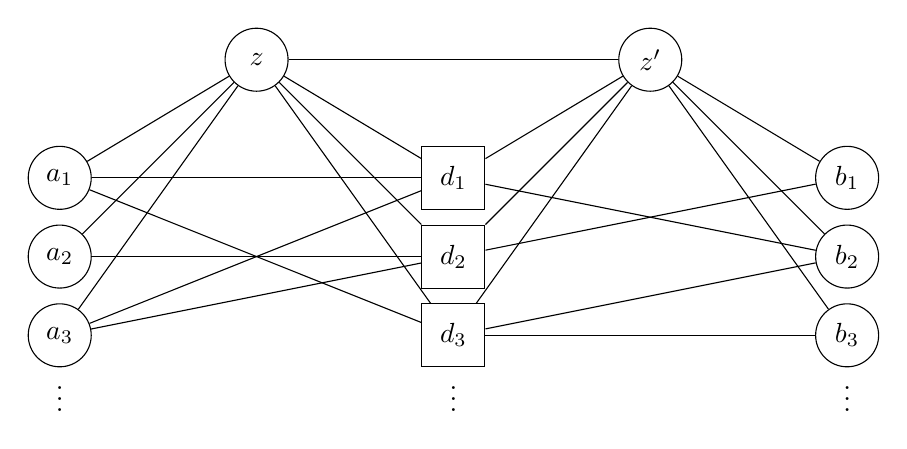
\begin{tikzpicture}[
				vertex/.style={circle, draw, minimum size=0.8cm, inner sep=0pt},
				dim/.style={rectangle, draw, minimum size=0.8cm, inner sep=0pt},
			]
			% z between A and D; z' between D and B; z--z' connected
			\node[vertex] (z)  at (2.5, 4)  {$z$};
			\node[vertex] (zp) at (7.5, 4)  {$z'$};

			% A column
			\node[vertex] (a1) at (0, 2.5)  {$a_1$};
			\node[vertex] (a2) at (0, 1.5)  {$a_2$};
			\node[vertex] (a3) at (0, 0.5)  {$a_3$};
			\node         (ad) at (0, -0.2) {$\vdots$};

			% Dimension column
			\node[dim]    (d1) at (5, 2.5)  {$d_1$};
			\node[dim]    (d2) at (5, 1.5)  {$d_2$};
			\node[dim]    (d3) at (5, 0.5)  {$d_3$};
			\node         (dd) at (5, -0.2) {$\vdots$};

			% B column
			\node[vertex] (b1) at (10, 2.5) {$b_1$};
			\node[vertex] (b2) at (10, 1.5) {$b_2$};
			\node[vertex] (b3) at (10, 0.5) {$b_3$};
			\node         (bd) at (10, -0.2){$\vdots$};

			% z -- z'
			\draw (z) -- (zp);

			% A to z
			\draw (a1) -- (z); \draw (a2) -- (z); \draw (a3) -- (z);

			% B to z'
			\draw (b1) -- (zp); \draw (b2) -- (zp); \draw (b3) -- (zp);

			% Dimension vertices to z and z'
			\draw (d1) -- (z);  \draw (d2) -- (z);  \draw (d3) -- (z);
			\draw (d1) -- (zp); \draw (d2) -- (zp); \draw (d3) -- (zp);

			% a_1=[1,0,1]: connects to d_1, d_3
			\draw (a1) -- (d1);
			\draw (a1) -- (d3);
			% a_2=[0,1,0]: connects to d_2
			\draw (a2) -- (d2);
			% a_3=[1,1,0]: connects to d_1, d_2
			\draw (a3) -- (d1);
			\draw (a3) -- (d2);

			% b_1=[0,1,0]: connects to d_2 (orthogonal to a_1 => dist 3)
			\draw (b1) -- (d2);
			% b_2=[1,0,1]: connects to d_1, d_3
			\draw (b2) -- (d1);
			\draw (b2) -- (d3);
			% b_3=[0,0,1]: connects to d_3
			\draw (b3) -- (d3);
		\end{tikzpicture}
	\end{center}
	In this example $a_1=[1,0,1]$ and $b_1=[0,1,0]$ are orthogonal: they share no dimension vertex, so their shortest path $a_1\!\to\!z\!\to\!z'\!\to\!b_1$ (length~3) determines the diameter.

	We can see that the distance between $z$, $z'$ and the dimension vertices is at most 2, and the distance between any two vertices in $A$ and $B$ is at most 3. Furthermore, if there exists $a_i, b_{i'}$ so that they're connected to the same dimension vertex, then the distance between them are 2. Otherwise, the distance between them is 3. Therefore, the diameter of $G$ is 3 if and only if there exist $a \in A$ and $b \in B$ such that they are not connected to the same dimension vertex, which is equivalent to $\langle a, b \rangle = 0$.

	If we can solve Diameter in $O(n^{2-\varepsilon})$ time, then we can solve Orthogonal Vectors in $O((2N+d+2)^{2-\varepsilon}) = O(N^{2-\varepsilon} \cdot \poly(d))$ time, which contradicts the assumption.
\end{proof}

\section{Regular Expression Matching}

\begin{problem}[Regular Expression Matching]
A \textbf{regular expression} is a string that describes a language. It can be defined recursively as follows:
\begin{itemize}
	\item $a\in \Sigma$ matches ``a'';
	\item $R_1R_2$ matches $s_1s_2$, where $R_1$ matches $s_1$ and $R_2$ matches $s_2$;
	\item $R_1|R_2$ matches $s$ if $s$ matches either $R_1$ or $R_2$;
	\item $R^*$ matches $\exists k \ge 0, s = s_1s_2\cdots s_k$ where $\forall i, s_i$ matches $R$.
\end{itemize}
Given a text $T \in \Sigma^*$ and a regular expression $R$, determine if $T$ matches $R$.
\end{problem}
\begin{theorem}
	If no algorithm can solve Orthogonal Vectors in $O(N^{2-\varepsilon} \cdot \poly(d))$ time for any $\varepsilon > 0$, then there is no algorithm that can solve Regular Expression Matching in $O((|T||R|)^{1-\varepsilon})$ time for any $\varepsilon > 0$.
\end{theorem}
\begin{proof}
	We construct a reduction from Orthogonal Vectors to Regular Expression Matching. Given two sets $A, B \subseteq \{0, 1\}^d$ of size $N$, we create a text $T$ and a regular expression $R$ as follows:
	\begin{itemize}
		\item $\Sigma = \{0, 1, \#\}$.
		\item $T = a_1\#a_2\#\cdots \#a_N\#$, where $a_i$ is the binary string corresponding to the vector $a_i \in A$.
		\item Construct $R(b_i)$ as follows: if $b_i[j] = 1$, then $R(b_i)[j] = 0$; if $b_i[j] = 0$, then $R(b_i)[j] = (0|1)$. Then, let $R = (0|1|\#)^*R(b_1)|R(b_2)|\cdots |R(b_N)(0|1|\#)^*$.
	\end{itemize}
	We can see that $T$ matches $R$ if and only if there exists $b_i \in B$ such that $R(b_i)$ matches some $a_j$ in $T$, which is equivalent to $\langle a_j, b_i \rangle = 0$.

	If we can solve Regular Expression Matching in $O((|T||R|)^{1-\varepsilon})$ time, then we can solve Orthogonal Vectors in $O(((Nd) \cdot (Nd))^{1-\varepsilon}) = O(N^{2-2\varepsilon} \cdot \poly(d))$ time, which contradicts the assumption.
\end{proof}
